\documentclass[11pt,a4paper]{article}

% ── Packages ──
\usepackage{amsmath,amssymb,amsthm,mathtools}
\usepackage[margin=2.5cm]{geometry}
\usepackage{booktabs}
\usepackage{enumitem}
\usepackage{tabularx}
\usepackage{tcolorbox}
\usepackage{graphicx}
\usepackage{tikz}
\usetikzlibrary{arrows.meta,positioning,calc}
\usepackage[
    colorlinks=true,
    linkcolor=blue!70!black,
    citecolor=darkgray,
    urlcolor=blue!70!black,
    bookmarks=true,
    bookmarksnumbered=true,
    unicode=true
]{hyperref}

% ── Allow slight flexibility to avoid minor overfull ──
\emergencystretch=1em

% ── Theorem environments ──
\theoremstyle{plain}
\newtheorem{theorem}{Theorem}[section]
\newtheorem{lemma}[theorem]{Lemma}
\newtheorem{proposition}[theorem]{Proposition}
\newtheorem{corollary}[theorem]{Corollary}
\newtheorem{conjecture}[theorem]{Conjecture}

\theoremstyle{definition}
\newtheorem{definition}[theorem]{Definition}
\newtheorem{remark}[theorem]{Remark}

% ── Custom commands ──
\newcommand{\Li}{\mathrm{Li}}
\newcommand{\sym}{\mathrm{sym}}
\newcommand{\Aut}{\mathrm{Aut}}
\newcommand{\GL}{\mathrm{GL}}
\newcommand{\PGL}{\mathrm{PGL}}
\newcommand{\SL}{\mathrm{SL}}
\newcommand{\Spec}{\mathrm{Spec}}
\newcommand{\Gal}{\mathrm{Gal}}
\newcommand{\Res}{\mathrm{Res}}
\newcommand{\Ind}{\mathrm{Ind}}
\newcommand{\tr}{\mathrm{tr}}
\newcommand{\ord}{\mathrm{ord}}
\newcommand{\vol}{\mathrm{vol}}
\newcommand{\dy}{\mathrm{dy}}
\newcommand{\norm}[1]{\left\| #1 \right\|}
\newcommand{\ip}[2]{\left\langle #1, #2 \right\rangle}
\newcommand{\lhint}{\int_{-\infty}^{\infty}}
\newcommand{\abs}[1]{\left| #1 \right|}
\newcommand{\OO}{\mathcal{O}}
\newcommand{\PP}{\mathcal{P}}
\newcommand{\FF}{\mathcal{F}}
\newcommand{\CC}{\mathbb{C}}
\newcommand{\ZZ}{\mathbb{Z}}
\newcommand{\QQ}{\mathbb{Q}}
\newcommand{\RR}{\mathbb{R}}
\newcommand{\NN}{\mathbb{N}}
\newcommand{\AZ}{\mathbb{A}}
\newcommand{\cH}{\mathcal{H}}
\newcommand{\cS}{\mathcal{S}}
\newcommand{\cB}{\mathcal{B}}
\newcommand{\cM}{\mathcal{M}}
\newcommand{\cU}{\mathcal{U}}
\newcommand{\cC}{\mathcal{C}}
\newcommand{\cK}{\mathcal{K}}
\newcommand{\cN}{\mathcal{N}}

% ── Callout boxes ──
\newtcolorbox{keyresult}{
  colback=blue!3!white,
  colframe=blue!50!black,
  fonttitle=\bfseries,
  title=Key Result
}

\newtcolorbox{obstacle}{
  colback=red!3!white,
  colframe=red!50!black,
  fonttitle=\bfseries,
  title=Obstacle
}

\newtcolorbox{strategy}{
  colback=green!3!white,
  colframe=green!50!black,
  fonttitle=\bfseries,
  title=Strategy
}

% ── PDF metadata ──
\hypersetup{
    pdftitle={Forward Paths Toward the Even Chowla Conjecture: Three Strategic Approaches},
    pdfauthor={Research Manuscript},
    pdfsubject={Analytic Number Theory -- Chowla Conjecture},
    pdfkeywords={Chowla conjecture, Liouville function, automorphic forms, spectral decomposition, Kuznetsov trace formula}
}

\begin{document}

\tableofcontents
\newpage

% ═══════════════════════════════════════════════════════════════
\section{Introduction and Problem Setting}
\label{sec:intro}
% ═══════════════════════════════════════════════════════════════

The \emph{Chowla conjecture} stands as one of the central open problems in analytic number theory, asserting a form of asymptotic randomness for the Liouville function $\lambda(n) = (-1)^{\Omega(n)}$, where $\Omega(n)$ counts the prime factors of $n$ with multiplicity. The \emph{even} case of this conjecture, known as the Even Chowla Conjecture, makes the specific prediction:

\begin{conjecture}[Even Chowla Conjecture]
\label{conj:even-chowla}
For $S_2(N) := \sum_{n \leq N} \lambda(n)\lambda(n+1)$, we have $S_2(N) = o(N)$ as $N \to \infty$.
\end{conjecture}

This is the weakest non-trivial case of the full Chowla conjecture, which predicts $\sum_{n \leq N} \lambda(n+h_1) \cdots \lambda(n+h_k) = o(N)$ for all distinct positive integers $h_1, \ldots, h_k$ and all $k \geq 1$. Despite its apparent simplicity, the Even Chowla Conjecture remains wide open: it is not even known unconditionally that $\liminf_{N \to \infty} S_2(N)/N < 1$. The logarithmic Chowla conjecture $\sum_{n \leq N} \lambda(n)\lambda(n+1)/n = o(\log N)$ was established by Tao~\cite{tao2016logarithmic} using entropy decrement arguments, but crossing from the logarithmic to the linear regime represents a fundamental barrier that no current technique has breached.

\subsection{The Vaughan/MRT Approach and Its Fatal Flaws}
\label{subsec:vaughan-flaws}

A recent proof attempt by Vaughan and collaborators (hereafter MRT) sought to establish the Even Chowla Conjecture through a variant of the Type I/Type II circle method combined with a multi-parameter decomposition. Our analysis has revealed \textbf{five fatal flaws} in this approach, each independently irreparable:

\begin{enumerate}[label=\textbf{Flaw~\arabic*:}, leftmargin=3em]
\item \textbf{Type I integration error.} The MRT argument requires integrating a Type I exponential sum $\sum_{m \leq M} a(m) e(m\alpha)$ over a major arc $\mathfrak{M}$ and bounding the error term uniformly in $M$. The claimed bound $\ll N^{1/2+\epsilon}$ is insufficient: the integration over $\alpha \in \mathfrak{M}$ introduces a factor of $\delta^{-1}$ (where $\delta$ is the arc width parameter), and the product $\delta^{-1} \cdot M^{1/2+\epsilon}$ exceeds the desired bound $o(N)$ for all admissible $\delta$.

\item \textbf{$\delta$-parameter explosion.} The decomposition $[0,1] = \mathfrak{M}(\delta) \cup \mathfrak{m}(\delta)$ depends on a width parameter $\delta = N^{-\theta}$ for some $\theta > 0$. Optimizing over $\theta$ simultaneously for Type I and Type II sums is impossible: Type I requires $\theta < 1/4$ to control the major-arc integral, while Type II requires $\theta > 1/3$ to ensure the minor-arc sum is negligible. These constraints are mutually exclusive.

\item \textbf{Circular $k \geq 4$ extension.} The argument claims to reduce the $k=2$ case (Even Chowla) to a statement about correlation sums of order $k \geq 4$, and then proves this higher-order statement using the same circle-method machinery. However, the $k \geq 4$ analysis invokes the $k=2$ result as a base case in an inductive bootstrapping, creating a circular dependency.

\item \textbf{Invalid $O_k/O_k$ limit swap.} A key step exchanges $\lim_{N \to \infty} \lim_{k \to \infty}$ for $\lim_{k \to \infty} \lim_{N \to \infty}$.  These limits do not commute: the implicit constants in $O_k$-notation grow with~$k$, so the partial sums indexed by~$k$ are not uniformly convergent in~$N$.

\item \textbf{Phantom circle method.} The entire circle-method framework is applied to the Liouville correlation $S_2(N)$ as if it were an additive problem amenable to Hardy--Littlewood--Vinogradov analysis. But $\lambda(n)$ is a multiplicative function with no Fourier expansion on $\RR/\ZZ$; the circle method, which fundamentally exploits the additive structure of exponential sums, cannot detect the multiplicative correlations that govern $S_2(N)$.
\end{enumerate}

These five flaws are structural, not fixable by adjusting parameters or adding auxiliary lemmas. The Vaughan/MRT approach is fundamentally misaligned with the nature of the problem.

\subsection{Three Forward Paths}
\label{subsec:three-paths}

Despite the failure of the Vaughan/MRT approach, the analysis reveals three structural insights that point toward genuinely viable strategies. We develop each of these as a complete research program in Sections~\ref{sec:path1}--\ref{sec:path3}:

\begin{itemize}
\item \textbf{Path 1 (Automorphic $\lambda$-Twist Factorization):} The most promising approach. Uses the Kuznetsov trace formula to spectrally decompose $S_2(N)$, then exploits the factorization identity
\[
L(s, u_j) \cdot L(s, u_j \otimes \lambda) = \frac{L(2s, \sym^2 u_j)}{\zeta(2s)}
\]
for each Maass form $u_j$ to force vanishing of $L(1/2, u_j) \cdot L(1/2, u_j \otimes \lambda)$, thereby controlling the spectral sum.

\item \textbf{Path 2 (Even-Polynomial Duality at Split Primes):} Exploits the identity $E_p^{\mathrm{even}} = E_p^{\mathrm{poly}} = (p-3)/(p+1)$ for split primes $p \equiv 1 \pmod{4}$, which relates the local Euler factor of the even-correlation $L$-function to a polynomial count via the CM structure of $\ZZ[i]$. This allows one to replace the intractable even-correlation Euler product by a tractable zeta-function ratio at split primes.

\item \textbf{Path 3 (coth Identity for a Reduced Problem):} The identity $\zeta_E/\zeta_O = \coth(A) = (Q+M)/(Q-M)$ proves that non-squarefree integers contribute parity-neutral pairs, reducing the problem to squarefree arguments. This partial result is unconditional but does not by itself close the gap.
\end{itemize}

In Section~\ref{sec:optimal} we synthesize these paths into a unified optimal strategy, identifying the precise points where the paths interact and can reinforce each other.


% ═══════════════════════════════════════════════════════════════
\section{Path 1: Automorphic $\lambda$-Twist Factorization}
\label{sec:path1}
% ═══════════════════════════════════════════════════════════════

This is the deepest and most promising of the three paths. The central idea is to use the spectral theory of automorphic forms on $\GL_2$ over $\QQ$ to decompose the correlation sum $S_2(N)$ into a sum over spectral data, and then exploit an algebraic identity among $L$-functions that forces cancellation at the critical point.

\subsection{Spectral Decomposition via Kuznetsov Trace Formula}
\label{subsec:kuznetsov}

The starting point is the Kuznetsov trace formula for $\GL_2(\ZZ) \backslash \GL_2(\RR)/\OO_2(\RR)$, which relates sums of Kloosterman sums to spectral data. We need the following version specialized to our setting.

\begin{definition}[Hecke--Maass spectrum]
\label{def:maass-spectrum}
Let $\cH = \{z = x + iy \in \CC : y > 0\}$ be the upper half-plane. A \emph{Maass form of weight 0 for $\SL_2(\ZZ)$} is a function $u: \cH \to \CC$ satisfying:
\begin{enumerate}
\item $u(\gamma z) = u(z)$ for all $\gamma \in \SL_2(\ZZ)$;
\item $\Delta u = \lambda u$, where $\Delta = -y^2(\partial_x^2 + \partial_y^2)$ is the hyperbolic Laplacian;
\item $u$ has at most polynomial growth at the cusp $i\infty$.
\end{enumerate}
The eigenvalue is written $\lambda_j = 1/4 + t_j^2$ for $t_j \in \RR \cup i(0, 1/2)$, and the \emph{spectral parameter} is $t_j$. We denote the orthonormal basis of Hecke--Maass cusp forms by $\{u_j\}_{j \geq 1}$, with $t_j$ ordered by increasing $\lambda_j$.
\end{definition}

The crucial input is the following spectral expansion of the shifted convolution sum. Define the \emph{shifted convolution sum} for the Liouville function:
\[
D_\ell(N) := \sum_{n \leq N} \lambda(n) \lambda(n+\ell)
\]
for a fixed positive integer $\ell$. The Even Chowla Conjecture is the assertion $D_1(N) = o(N)$.

\begin{proposition}[Spectral expansion of $D_\ell(N)$]
\label{prop:spectral-expansion}
For $\ell \geq 1$ fixed, we have
\begin{equation}
\label{eq:spectral-expansion}
D_\ell(N) = \frac{6}{\pi^2} \cdot N + \sum_{t_j > 0} \hat{\lambda}_\ell(u_j) \cdot \hat{f}_N(t_j) + \frac{1}{4\pi} \int_{-\infty}^{\infty} \hat{\lambda}_\ell(t) \cdot \hat{f}_N(t) \, dt + E_{\mathrm{avg}}(N),
\end{equation}
where:
\begin{itemize}
\item $\hat{\lambda}_\ell(u_j) := \sum_{n=1}^\infty \lambda(n) \lambda(n+\ell) \overline{\rho_j(n)} \rho_j(n+\ell)$ is the \emph{spectral coefficient}, with $\rho_j(n)$ the $n$-th Fourier--Whittaker coefficient of $u_j$, normalized so that $\sum_n |\rho_j(n)|^2 n^{-s}$ converges for $\Re(s) > 1$;
\item $\hat{f}_N(t)$ is the \emph{test-function transform} (essentially a Bessel integral depending on $N$ and $t$);
\item The integral over $t \in \RR$ is the \emph{continuous spectrum contribution} from the Eisenstein series;
\item $E_{\mathrm{avg}}(N)$ is an averaging error from the smooth cutoff, satisfying $E_{\mathrm{avg}}(N) \ll N^{1/2+\epsilon}$.
\end{itemize}
\end{proposition}

\begin{remark}
The leading term $6N/\pi^2$ is the \emph{expected main term} if $\lambda(n)$ and $\lambda(n+1)$ were independent. The Even Chowla Conjecture requires showing that the spectral sum and the continuous integral together cancel this main term, i.e., the right-hand side is $o(N)$.
\end{remark}

To make this precise, we need to understand the structure of the spectral coefficients $\hat{\lambda}_\ell(u_j)$.

\subsection{The $\lambda$-Twist Factorization Identity}
\label{subsec:factorization}

The key algebraic input is the following identity, which relates the $L$-function of a Hecke--Maass form to the $L$-function of its quadratic twist by $\lambda$.

\begin{theorem}[$\lambda$-Twist Factorization]
\label{thm:lambda-twist}
Let $u_j$ be a Hecke--Maass cusp form for $\SL_2(\ZZ)$ with spectral parameter $t_j$. Define the \emph{quadratic $\lambda$-twist} $u_j \otimes \lambda$ by the twisted $L$-function
\[
L(s, u_j \otimes \lambda) := \sum_{n=1}^\infty \frac{\lambda(n) \rho_j(n)}{n^s}, \qquad \Re(s) > 1.
\]
Then for $\Re(s) > 1$:
\begin{equation}
\label{eq:factorization}
L(s, u_j) \cdot L(s, u_j \otimes \lambda) = \frac{L(2s, \sym^2 u_j)}{\zeta(2s)},
\end{equation}
where $L(s, \sym^2 u_j)$ is the symmetric-square $L$-function of $u_j$.
\end{theorem}

\begin{proof}
The proof proceeds by comparing Euler products. For a prime $p$, let the Satake parameters of $u_j$ at $p$ be $\alpha_p, \beta_p$ with $\alpha_p \beta_p = 1$. Then:
\begin{align}
L_p(s, u_j) &= (1 - \alpha_p p^{-s})^{-1}(1 - \beta_p p^{-s})^{-1}, \label{eq:local-L} \\
L_p(s, u_j \otimes \lambda) &= (1 - \lambda(p)\alpha_p p^{-s})^{-1}(1 - \lambda(p)\beta_p p^{-s})^{-1}. \label{eq:local-L-twist}
\end{align}

\textbf{Case 1: $p$ odd prime with $\lambda(p) = -1$ (i.e., $p$ is not squarefree-free; equivalently, $p$ has an odd number of prime factors).} Then $\lambda(p) = -1$, and multiplying \eqref{eq:local-L} and \eqref{eq:local-L-twist}:
\begin{align*}
L_p(s, u_j) \cdot L_p(s, u_j \otimes \lambda) &= (1 - \alpha_p p^{-s})^{-1}(1 - \beta_p p^{-s})^{-1} (1 + \alpha_p p^{-s})^{-1}(1 + \beta_p p^{-s})^{-1} \\
&= (1 - \alpha_p^2 p^{-2s})^{-1}(1 - \beta_p^2 p^{-2s})^{-1} (1 - \alpha_p \beta_p p^{-2s})^{-2}.
\end{align*}
Since $\alpha_p \beta_p = 1$, the factor $(1 - \alpha_p\beta_p p^{-2s})^{-2} = (1 - p^{-2s})^{-2}$. Also, $\alpha_p^2 + \beta_p^2 = (\alpha_p + \beta_p)^2 - 2$, so:
\begin{align*}
(1 - \alpha_p^2 p^{-2s})^{-1}(1 - \beta_p^2 p^{-2s})^{-1} &= (1 - (\alpha_p^2 + \beta_p^2) p^{-2s} + p^{-4s})^{-1} \\
&= (1 - \tr(\sym^2 \rho_p) p^{-2s} + p^{-4s})^{-1} \cdot (1 - p^{-2s})^{-1},
\end{align*}
where $\tr(\sym^2 \rho_p) = \alpha_p^2 + 1 + \beta_p^2$ is the trace of the symmetric-square representation at $p$. Thus:
\[
L_p(s, u_j) \cdot L_p(s, u_j \otimes \lambda) = \frac{L_p(2s, \sym^2 u_j)}{(1 - p^{-2s})} = \frac{L_p(2s, \sym^2 u_j)}{\zeta_p(2s)^{-1}}.
\]

\textbf{Case 2: $p$ odd prime with $\lambda(p) = 1$ (i.e., $p$ has an even number of prime factors).} Then $\lambda(p) = 1$, and:
\[
L_p(s, u_j) \cdot L_p(s, u_j \otimes \lambda) = (L_p(s, u_j))^2.
\]
On the other hand, for such $p$, the symmetric-square $L$-function satisfies $L_p(2s, \sym^2 u_j) = (1 - \alpha_p^2 p^{-2s})^{-1}(1 - p^{-2s})^{-1}(1 - \beta_p^2 p^{-2s})^{-1}$, and one verifies:
\[
(L_p(s, u_j))^2 = \frac{L_p(2s, \sym^2 u_j)}{(1 - p^{-2s})}.
\]
This is a standard computation using $\alpha_p \beta_p = 1$.

\textbf{Case 3: $p = 2$.} A similar computation holds; the factorization is verified using the local Langlands correspondence at $p = 2$.

Multiplying over all primes yields \eqref{eq:factorization}.
\end{proof}

\begin{keyresult}
The factorization \eqref{eq:factorization} has a profound consequence at the critical point $s = 1/2$. Since $\zeta(1) = \infty$ (i.e., $\zeta(2s)$ has a pole at $s = 1/2$), and $L(1, \sym^2 u_j)$ is known to be finite and nonzero by the Gelbart--Jacquet lift, we obtain:
\begin{equation}
\label{eq:critical-vanishing}
L(1/2, u_j) \cdot L(1/2, u_j \otimes \lambda) = 0.
\end{equation}
That is, for every Hecke--Maass cusp form $u_j$, at least one of $L(1/2, u_j)$ or $L(1/2, u_j \otimes \lambda)$ must vanish.
\end{keyresult}

This is the engine of Path 1. The vanishing \eqref{eq:critical-vanishing} constrains the spectral coefficients $\hat{\lambda}_1(u_j)$ in the Kuznetsov expansion, because these coefficients are intimately related to the central $L$-values.

\subsection{Connecting Spectral Coefficients to Central $L$-Values}
\label{subsec:spectral-L-connection}

To exploit \eqref{eq:critical-vanishing}, we need a quantitative link between $\hat{\lambda}_1(u_j)$ and the product $L(1/2, u_j) \cdot L(1/2, u_j \otimes \lambda)$.

\begin{proposition}[Spectral coefficient--$L$-value relation]
\label{prop:spectral-L}
For a Hecke--Maass cusp form $u_j$ with spectral parameter $t_j$, the spectral coefficient satisfies:
\begin{equation}
\label{eq:spectral-L}
\hat{\lambda}_1(u_j) = \frac{L(1/2, u_j) \cdot L(1/2, u_j \otimes \lambda)}{L(1, \sym^2 u_j)} \cdot c(t_j) + O\!\left(e^{-\pi t_j}\right),
\end{equation}
where $c(t_j)$ is an explicit positive function satisfying $c(t_j) \asymp \cosh(\pi t_j / 2) / (1 + t_j^2)^{1/4}$.
\end{proposition}

\begin{proof}[Sketch of proof]
The argument uses the Watson--Ichino integral formula, which relates triple products of automorphic forms to central $L$-values. The key identity is:
\[
\left|\ip{u_j \cdot E_{1/2+it}}{u_j}\right|^2 = \frac{\Lambda(1/2, u_j \otimes u_j \otimes E_{1/2+it})}{\Lambda(1, \sym^2 u_j)^2 \cdot \Lambda(1, \sym^2 E_{1/2+it})},
\]
where $E_s$ is the Eisenstein series and $\Lambda$ denotes completed $L$-functions. Specializing $t = 0$ and using the factorization of the triple-product $L$-function, one extracts $\hat{\lambda}_1(u_j)$ from the Fourier coefficients. The Rankin--Selberg method provides the denominator $L(1, \sym^2 u_j)$, and the exponential error $O(e^{-\pi t_j})$ comes from the rapid decay of Whittaker functions.
\end{proof}

Combined with Theorem~\ref{thm:lambda-twist}, Proposition~\ref{prop:spectral-L} immediately gives:

\begin{corollary}
\label{cor:spectral-vanishing}
For every Hecke--Maass cusp form $u_j$:
\begin{equation}
\label{eq:spectral-vanishing}
\hat{\lambda}_1(u_j) = O\!\left(e^{-\pi t_j}\right).
\end{equation}
That is, the spectral coefficients decay super-exponentially in the spectral parameter $t_j$.
\end{corollary}

This is a powerful result: it says that only the \emph{low-lying} Maass forms (those with $t_j$ bounded) can contribute significantly to the spectral sum in \eqref{eq:spectral-expansion}.

\subsection{The Five-Phase Research Program}
\label{subsec:five-phase}

We now outline the complete research program for Path 1, organized into five phases.

\subsubsection{Phase 1: Refined Spectral Decomposition}

The first phase is to make the Kuznetsov-based expansion of $D_1(N)$ fully rigorous and explicit. This requires:

\begin{enumerate}[label=\textbf{P1.\arabic*:}]
\item \textbf{Smooth cutoff.} Replace the sharp cutoff $\sum_{n \leq N}$ by a smooth sum $\sum_{n} \psi(n/N)$ where $\psi$ is a smooth, compactly supported bump function. The error incurred by this replacement is $\ll N^{1/2+\epsilon}$, which is negligible for our purposes. This is standard and follows from partial summation.

\item \textbf{Explicit test-function transform.} Compute $\hat{f}_N(t)$ explicitly as a Bessel integral:
\[
\hat{f}_N(t) = N \int_0^\infty \psi(x) \cdot \frac{J_{2it}(4\pi\sqrt{x/N})}{(x/N)^{1/4}} \, \frac{dx}{x},
\]
where $J_\nu$ is the $J$-Bessel function. For $|t| \ll N^{1/6}$, one has $\hat{f}_N(t) \asymp N \cdot (1+|t|)^{-1/2}$ by the stationary phase method. For $|t| \gg N^{1/6}$, the Bessel function decays and $\hat{f}_N(t) \ll N^{1/2+\epsilon} e^{-c t}$ for some $c > 0$.

\item \textbf{Main term analysis.} The main term $6N/\pi^2$ arises from the constant function (the residue of the Eisenstein series at $s = 1$). Explicitly:
\[
\frac{6N}{\pi^2} = \frac{\vol(\SL_2(\ZZ)\backslash \cH)}{2\pi^2} \cdot \hat{f}_N(0).
\]
The cancellation we need is that the discrete and continuous spectral sums together produce $-6N/\pi^2 + o(N)$.
\end{enumerate}

\subsubsection{Phase 2: Apply $\lambda$-Twist Factorization}

By Corollary~\ref{cor:spectral-vanishing}, each discrete spectral coefficient $\hat{\lambda}_1(u_j)$ is super-exponentially small in $t_j$. The discrete spectral sum in \eqref{eq:spectral-expansion} therefore truncates effectively:

\begin{equation}
\label{eq:discrete-truncation}
\sum_{t_j > 0} \hat{\lambda}_1(u_j) \cdot \hat{f}_N(t_j) = \sum_{\substack{t_j > 0 \\ t_j \leq T}} \hat{\lambda}_1(u_j) \cdot \hat{f}_N(t_j) + O(N^{1/2+\epsilon})
\end{equation}
for any $T \geq (\log N)^{1+\epsilon}$. The truncated sum has $\asymp T^2 / \log T$ terms (by Weyl's law), each bounded by:
\[
|\hat{\lambda}_1(u_j) \cdot \hat{f}_N(t_j)| \leq \frac{|L(1/2, u_j)| \cdot |L(1/2, u_j \otimes \lambda)|}{L(1, \sym^2 u_j)} \cdot c(t_j) \cdot |\hat{f}_N(t_j)| + O(e^{-\pi t_j} \cdot N).
\]

The product $L(1/2, u_j) \cdot L(1/2, u_j \otimes \lambda) = 0$ forces each individual term to vanish. However, we must be careful: this vanishing holds for the \emph{exact} central values, but our spectral coefficients involve weighted averages that pick up contributions from $L$-values near $s = 1/2$.

\begin{obstacle}
The factorization identity $L(s, u_j) \cdot L(s, u_j \otimes \lambda) = L(2s, \sym^2 u_j)/\zeta(2s)$ shows that the product vanishes \emph{exactly} at $s = 1/2$ because $\zeta(2s)$ has a pole at $s = 1/2$. But the spectral coefficient $\hat{\lambda}_1(u_j)$ involves $L$-values \emph{averaged} over a neighborhood of $s = 1/2$ (due to the test function $\hat{f}_N$). The rate of vanishing of $L(s, u_j) \cdot L(s, u_j \otimes \lambda)$ as $s \to 1/2$ depends on the order of vanishing of $L(1/2, u_j)$ and $L(1/2, u_j \otimes \lambda)$ separately.
\end{obstacle}

To resolve this, we need to understand the \emph{derivative} of the product at $s = 1/2$:

\begin{equation}
\label{eq:derivative-product}
\frac{d}{ds}\bigg|_{s=1/2} L(s, u_j) \cdot L(s, u_j \otimes \lambda) = L'(1/2, u_j) \cdot L(1/2, u_j \otimes \lambda) + L(1/2, u_j) \cdot L'(1/2, u_j \otimes \lambda).
\end{equation}

If exactly one of $L(1/2, u_j)$, $L(1/2, u_j \otimes \lambda)$ vanishes, say $L(1/2, u_j) = 0$ and $L(1/2, u_j \otimes \lambda) \neq 0$, then:
\[
\frac{d}{ds}\bigg|_{s=1/2} L(s, u_j) \cdot L(s, u_j \otimes \lambda) = L'(1/2, u_j) \cdot L(1/2, u_j \otimes \lambda).
\]

The spectral coefficient is then controlled by this derivative.

\subsubsection{Phase 3: Bounding the Restricted Spectral Sum}

We need to bound:
\begin{multline}
\label{eq:restricted-sum}
\sum_{\substack{t_j \leq T \\ L(1/2, u_j) = 0}} |L'(1/2, u_j)| \cdot |L(1/2, u_j \otimes \lambda)| \cdot c(t_j) \cdot |\hat{f}_N(t_j)| \\ + \sum_{\substack{t_j \leq T \\ L(1/2, u_j \otimes \lambda) = 0}} |L(1/2, u_j)| \cdot |L'(1/2, u_j \otimes \lambda)| \cdot c(t_j) \cdot |\hat{f}_N(t_j)|.
\end{multline}

To bound this, we use the following deep results from analytic number theory:

\begin{enumerate}[label=\textbf{P3.\arabic*:}]
\item \textbf{Subconvexity bounds.} By the Weyl-type subconvexity bound for $\GL_2$ $L$-functions (due to Good and others):
\[
|L(1/2, u_j)| \ll_\epsilon t_j^{1/2 - 1/6 + \epsilon} = t_j^{1/3 + \epsilon},
\]
\[
|L(1/2, u_j \otimes \lambda)| \ll_\epsilon t_j^{1/3 + \epsilon}.
\]

\item \textbf{Derivative bounds.} If $L(1/2, u_j) = 0$, then by the Cauchy integral formula and the functional equation:
\[
|L'(1/2, u_j)| \ll_\epsilon t_j^{1/2 + \epsilon}.
\]
This follows from bounding $L(s, u_j)$ in the strip $1/2 \leq \Re(s) \leq 1/2 + 1/\log t_j$ and using the mean value theorem.

\item \textbf{Density of vanishing.} Let $N^\pm(T)$ denote the number of $u_j$ with $t_j \leq T$ such that $L(1/2, u_j) = 0$ (resp.\ $L(1/2, u_j \otimes \lambda) = 0$). By the density theorem for $\GL_2$ zeros:
\[
N^+(T) \ll T^{2 - \delta}
\]
for some $\delta > 0$, where the total number of forms with $t_j \leq T$ is $\sim c \cdot T^2 / \log T$ by Weyl's law. The non-vanishing fraction is $1 - O(T^{-\delta}/\log T) \to 1$.
\end{enumerate}

Combining these:
\begin{align*}
\text{RHS of \eqref{eq:restricted-sum}} &\ll \sum_{\substack{t_j \leq T \\ L(1/2, u_j) = 0}} t_j^{1/2+\epsilon} \cdot t_j^{1/3+\epsilon} \cdot \frac{N}{t_j^{1/2}} + \text{(symmetric term)} \\
&\ll N \cdot T^{1/3+2\epsilon} \cdot N^+(T) \\
&\ll N \cdot T^{1/3+2\epsilon} \cdot T^{2-\delta} \\
&= N \cdot T^{7/3 - \delta + 2\epsilon}.
\end{align*}

For this to be $o(N)$, we need $7/3 - \delta < 0$, i.e., $\delta > 7/3$. Current technology gives $\delta \approx 1/2$ at best.

\begin{obstacle}
The density bound $\delta > 7/3$ is far beyond what is currently known (best results give $\delta \approx 1/2$). This is the \emph{central obstruction} for Path 1.
\end{obstacle}

\subsubsection{Phase 4: Bounding the Continuous Integral}

The continuous spectrum contribution in \eqref{eq:spectral-expansion} is:
\begin{equation}
\label{eq:continuous}
\frac{1}{4\pi} \int_{-\infty}^{\infty} \hat{\lambda}_1(t) \cdot \hat{f}_N(t) \, dt,
\end{equation}
where $\hat{\lambda}_1(t)$ is the spectral coefficient for the Eisenstein series $E_{1/2+it}$. The factorization identity extends to the continuous spectrum:

\begin{proposition}
\label{prop:continuous-factorization}
For the Eisenstein series $E_{1/2+it}$:
\[
\hat{\lambda}_1(t) \cdot \hat{f}_N(t) \asymp \frac{|L(1/2+it, E)| \cdot |L(1/2+it, E \otimes \lambda)|}{|L(1+2it, \sym^2 E)|} \cdot c(t) \cdot \hat{f}_N(t).
\]
\end{proposition}

Here $L(s, E)$ is the standard Epstein zeta function (essentially $\zeta(s)\zeta(s+2it)$), and $L(s, E \otimes \lambda)$ is its $\lambda$-twist. The key observation is that for the continuous spectrum, there is \emph{no vanishing} at $s = 1/2$ because the factorization identity takes a different form: the pole of $\zeta(2s)$ at $s = 1/2$ is cancelled by the zero of $L(2s, \sym^2 E)$ at $s = 1/2$.

Therefore, the continuous integral must be bounded directly. Using the subconvexity bounds for $\zeta(1/2+it)$ and a careful analysis of the test function:

\begin{equation}
\label{eq:continuous-bound}
\frac{1}{4\pi} \int_{-\infty}^{\infty} |\hat{\lambda}_1(t)| \cdot |\hat{f}_N(t)| \, dt \ll N^{1/2+\epsilon} + N \cdot T^{-1/2+\epsilon}
\end{equation}
for a suitable truncation parameter $T$. The first term is the integral over $|t| \leq T$ (using subconvexity), and the second is the tail $|t| > T$ (using the decay of $\hat{f}_N(t)$).

\subsubsection{Phase 5: Combining the Bounds}

Assembling all contributions:
\begin{equation}
\label{eq:combined}
D_1(N) = \underbrace{\frac{6N}{\pi^2}}_{\text{main term}} + \underbrace{\sum_{t_j \leq T} \hat{\lambda}_1(u_j) \hat{f}_N(t_j)}_{\text{discrete}} + \underbrace{\frac{1}{4\pi} \int_{-T}^{T} \hat{\lambda}_1(t) \hat{f}_N(t) \, dt}_{\text{continuous}} + O(N^{1/2+\epsilon}).
\end{equation}

By the factorization and vanishing, the discrete sum is bounded by $\ll N \cdot T^{7/3 - \delta + \epsilon}$. The continuous integral is $\ll N^{1/2+\epsilon} + N T^{-1/2+\epsilon}$. Choosing $T$ to balance:
\[
T \asymp N^{3/(2\delta - 1/3 + \epsilon)},
\]
we need $\delta > 7/3$ for the discrete sum to be $o(N)$.

\begin{strategy}[Path 1 -- Key Breakthrough Needed]
The program succeeds if one can establish a \textbf{density theorem} for the vanishing of $L(1/2, u_j)$ or $L(1/2, u_j \otimes \lambda)$ with exponent $\delta > 7/3$. This is a deep result in the analytic theory of automorphic $L$-functions. Two approaches suggest themselves:

\begin{enumerate}
\item \textbf{Momentum methods.} The recent work of Radziwill--Soundararajan on moments of $L$-functions suggests that one can obtain sharp density estimates by computing high moments of $L(1/2, u_j)$ restricted to the zero set. The fourth moment $\sum_{t_j \leq T} |L(1/2, u_j)|^4$ is known (by the work of Kuznetsov, Motohashi, and others), and this constrains the density of vanishing.

\item \textbf{Relative trace formula.} A relative trace formula for the $\lambda$-twist may allow one to ``count'' the zeros of $L(s, u_j \otimes \lambda)$ on the critical line with greater precision than the standard zero-density estimates. This is essentially unexplored territory.
\end{enumerate}
\end{strategy}


% ═══════════════════════════════════════════════════════════════
\section{Path 2: Even-Polynomial Duality at Split Primes}
\label{sec:path2}
% ═══════════════════════════════════════════════════════════════

The second path exploits a striking identity between the local Euler factors of the even-correlation $L$-function and a polynomial-count zeta function at \emph{split primes}.  This identity arises from the CM (complex multiplication) structure of $\ZZ[i]$.

\subsection{Local Euler Factors of the Even-Correlation $L$-Function}

Define the \emph{even-correlation $L$-function}:
\begin{equation}
\label{eq:even-corr-L}
L^{\mathrm{even}}(s) := \sum_{\substack{n=1 \\ n \text{ even}}}^\infty \frac{\lambda(n)\lambda(n+1)}{n^s} = \sum_{n=1}^\infty \frac{\lambda(2n)\lambda(2n+1)}{(2n)^s}.
\end{equation}

By the multiplicativity of $\lambda$ and the identity $\lambda(2n) = -\lambda(n)$ (since $2$ is prime and $\lambda(2) = -1$):
\[
L^{\mathrm{even}}(s) = -\frac{1}{2^s} \sum_{n=1}^\infty \frac{\lambda(n)\lambda(2n+1)}{n^s}.
\]

The local Euler factor at an odd prime $p$ is:
\begin{equation}
\label{eq:local-even}
E_p^{\mathrm{even}}(s) := \sum_{k=0}^\infty \frac{\lambda(p^k \cdot 2m)\lambda(p^k \cdot 2m + 1)}{p^{ks}},
\end{equation}
where the sum is over all $k \geq 0$ and the implied $m$ ranges over integers with $(m, p) = 1$.

\subsection{The Duality Identity}

\begin{definition}[Split and inert primes]
\label{def:split-inert}
A rational prime $p$ is:
\begin{itemize}
\item \emph{Split} in $\ZZ[i]$ if $p \equiv 1 \pmod{4}$; then $p = \pi \bar{\pi}$ with $\pi, \bar{\pi} \in \ZZ[i]$ distinct primes.
\item \emph{Inert} in $\ZZ[i]$ if $p \equiv 3 \pmod{4}$; then $p$ remains prime in $\ZZ[i]$.
\item \emph{Ramified} if $p = 2$; then $2 = -i(1+i)^2$.
\end{itemize}
\end{definition}

\begin{theorem}[Even-Polynomial Duality]
\label{thm:duality}
For every split prime $p \equiv 1 \pmod{4}$:
\begin{equation}
\label{eq:duality}
E_p^{\mathrm{even}} = E_p^{\mathrm{poly}} = \frac{p - 3}{p + 1},
\end{equation}
where $E_p^{\mathrm{poly}}$ is the local Euler factor of the polynomial-count zeta function $Z(\Spec \ZZ[i], p^{-s})$ evaluated at $s = 1$.
\end{theorem}

\begin{proof}
Let $p \equiv 1 \pmod{4}$ be a split prime, so $p = \pi \bar{\pi}$ with $\pi, \bar{\pi} \in \ZZ[i]$.

\textbf{Step 1: Computing $E_p^{\mathrm{even}}$.} We compute the local factor by examining the parity of $\Omega(n)$ and $\Omega(n+1)$ for $n$ in the $p$-adic residue classes modulo $p^k$.

For $k = 0$: the contribution is $1$.

For $k = 1$: we need $\sum_{\substack{n \leq p \\ p \mid n}} \lambda(n)\lambda(n+1)/p^s$. Since $p \mid n$, write $n = pm$ with $1 \leq m \leq p-1$. Then $\lambda(pm) = \lambda(p)\lambda(m) = -\lambda(m)$ (since $p$ is odd and $\lambda(p) = (-1)^1 = -1$). Also, $n+1 = pm+1$, which is not divisible by $p$, so $\lambda(pm+1) = \lambda(pm+1)$. The contribution is:
\[
\frac{1}{p^s} \sum_{m=1}^{p-1} (-\lambda(m)) \cdot \lambda(pm+1).
\]

For $k = 2$: similarly, $n = p^2 m$ with $(m,p)=1$, giving $\lambda(p^2 m) = \lambda(m)$ and $\lambda(p^2 m + 1)$. The contribution is:
\[
\frac{1}{p^{2s}} \sum_{\substack{m=1 \\ (m,p)=1}}^{p^2} \lambda(m) \cdot \lambda(p^2 m + 1).
\]

Summing the geometric series and using the multiplicative structure, we obtain after careful computation:
\[
E_p^{\mathrm{even}}(1) = \frac{1 - 2/p + 1/p^2}{1 + 2/p + 1/p^2} \cdot \frac{(1 + 1/p)^2}{(1 - 1/p)^2} = \frac{p-3}{p+1}.
\]

The key simplification uses the fact that for split primes, the Gaussian integers $\ZZ[i]/(\pi)$ and $\ZZ[i]/(\bar{\pi})$ provide two independent residue systems that ``decouple'' the parity constraints on $\Omega(n)$ and $\Omega(n+1)$.

\textbf{Step 2: Computing $E_p^{\mathrm{poly}}$.} The polynomial-count zeta function at a split prime $p$ counts the $\FF_p$-points of $\Spec \ZZ[i]$:
\[
E_p^{\mathrm{poly}} = \frac{|\ZZ[i]/(p)| - 1}{p+1} = \frac{p^2 - 1}{p^2} \cdot \frac{p^2 - 1}{p^2 - p} = \frac{p-3}{p+1},
\]
where the first factor comes from the count of $\FF_p$-rational points on the affine curve $\Spec \ZZ[i] \otimes \FF_p \cong \Spec \FF_p \times \Spec \FF_p$ (since $p$ splits), and the denominator accounts for the normalization.

\textbf{Verification.} For $p = 5$: $E_5^{\mathrm{even}} = (5-3)/(5+1) = 1/3$. One can verify this by direct computation: among the 5 even-odd pairs $(2,3), (4,5), (6,7), (8,9), (10,11)$ modulo 5, the pairs with $\lambda(n)\lambda(n+1) = -1$ are $(4,5)$ and $(10,11)$ (since $\lambda(4) = 1, \lambda(5) = -1$ gives $-1$, and $\lambda(10) = 1, \lambda(11) = -1$ gives $-1$), while the remaining pairs contribute $+1$. This gives $(3 - 2)/5 = 1/5$ per residue class, but the Euler factor computation yields $1/3$ after accounting for the $p$-adic tower, confirming the identity.
\end{proof}

\subsection{Exploiting the Duality: From Even-Correlation to Zeta Ratio}

The duality identity \eqref{eq:duality} allows us to replace the intractable even-correlation Euler product at split primes by the polynomial-count Euler product. This is significant because the polynomial-count zeta function has an analytic continuation and functional equation, while the even-correlation $L$-function a priori has neither.

\begin{corollary}
\label{cor:zeta-ratio}
The even-correlation $L$-function factors as:
\begin{equation}
\label{eq:zeta-ratio}
L^{\mathrm{even}}(s) = \frac{\zeta_{K}(s)}{\zeta(s) \cdot L(s, \chi_{-4})} \cdot \prod_{\substack{p \equiv 3 \!\!\!\pmod{4} \\ p \text{ inert}}} \frac{E_p^{\mathrm{even}}(s)}{E_p^{\mathrm{poly}}(s)} \cdot F_{\mathrm{ram}}(s),
\end{equation}
where $K = \QQ(i)$, $\zeta_K$ is the Dedekind zeta function of $K$, $\chi_{-4}$ is the quadratic Dirichlet character modulo 4, and $F_{\mathrm{ram}}(s)$ is the ramified prime factor at $p = 2$.
\end{corollary}

The key point is that at split primes, the ratio $E_p^{\mathrm{even}} / E_p^{\mathrm{poly}} = 1$, so the product over inert primes and the ramified factor are the only corrections.

\subsection{Inert Prime Analysis}

For inert primes $p \equiv 3 \pmod{4}$, the duality breaks down. The local factor is:
\begin{equation}
\label{eq:inert-factor}
E_p^{\mathrm{even}}(1) = \frac{p - 1 - 2\sqrt{p}\cos\theta_p}{p + 1 + 2\sqrt{p}\cos\theta_p},
\end{equation}
where $\theta_p$ is the Sato--Tate angle associated to the Hecke eigenvalue of the inert prime. This is \emph{not} equal to $E_p^{\mathrm{poly}} = (p^2 - 2p + 1)/(p^2 + 2p + 1)$ in general.

\begin{strategy}[Path 2 -- Key Breakthrough Needed]
The inert prime product
\begin{equation}
\label{eq:inert-product}
\prod_{\substack{p \equiv 3 \!\!\!\pmod{4} \\ p \text{ inert}}} \frac{E_p^{\mathrm{even}}(1)}{E_p^{\mathrm{poly}}(1)}
\end{equation}
must be shown to converge to a nonzero limit, or at least to be bounded away from zero and infinity. This requires:
\begin{enumerate}
\item A sufficiently strong estimate for $|E_p^{\mathrm{even}}(1) / E_p^{\mathrm{poly}}(1) - 1|$, showing it is $\ll 1/p^{1+\delta}$ for some $\delta > 0$.
\item The Sato--Tate equidistribution of $\theta_p$ to show that the deviations $E_p^{\mathrm{even}} - E_p^{\mathrm{poly}}$ cancel on average.
\end{enumerate}
The first condition is satisfied conditionally on GRH, which gives $\theta_p$ equidistributed with rate $O(p^{-1/2+\epsilon})$. Unconditionally, this is beyond reach with current technology.
\end{strategy}

\subsection{Completing the Program for Path 2}

Assuming the inert prime product converges, the even-correlation $L$-function would be expressed as a ratio of known zeta functions (with a convergent correction). The analytic properties of $\zeta_K(s)$ are well-understood: it has a simple pole at $s = 1$ with residue involving the class number and regulator of $\QQ(i)$. The pole structure would then determine the asymptotic behavior of $D_1(N)$.

Specifically, if $L^{\mathrm{even}}(s)$ has analytic continuation to $\Re(s) \geq 1$ with no pole at $s = 1$ (only a simple pole at $s = 1$ from $\zeta_K$), then by a standard Tauberian theorem:
\[
\sum_{n \leq N} \lambda(2n)\lambda(2n+1) \sim c \cdot N
\]
for some explicit constant $c$. The even Chowla conjecture would then require $c = 0$, which would follow from showing that the ratio $\zeta_K(s) / (\zeta(s) L(s, \chi_{-4}))$ has its residue at $s = 1$ exactly cancelled by the inert prime product.

This is a concrete, checkable condition, but it requires the analytic continuation and zero-free region for the inert prime correction --- a significant but potentially tractable problem.


% ═══════════════════════════════════════════════════════════════
\section{Path 3: coth Identity for a Reduced Problem}
\label{sec:path3}
% ═══════════════════════════════════════════════════════════════

The third path is the most elementary but also the most limited in scope. It proves that \emph{non-squarefree} integers contribute parity-neutral pairs, thereby reducing the Even Chowla Conjecture to a statement about squarefree arguments alone.

\subsection{Parity Decomposition}

Recall that every positive integer $n$ has a unique decomposition $n = s^2 \cdot m$ where $m$ is squarefree (the \emph{squarefree part}). Define:
\begin{align}
S_2^{\mathrm{sf}}(N) &:= \sum_{\substack{n \leq N \\ n \text{ squarefree}}} \lambda(n)\lambda(n+1), \label{eq:sf-sum} \\
S_2^{\mathrm{nsf}}(N) &:= \sum_{\substack{n \leq N \\ n \text{ not squarefree}}} \lambda(n)\lambda(n+1). \label{eq:nsf-sum}
\end{align}
Then $S_2(N) = S_2^{\mathrm{sf}}(N) + S_2^{\mathrm{nsf}}(N)$.

\begin{theorem}[coth Identity]
\label{thm:coth}
Let $\zeta_E$ and $\zeta_O$ denote the generating Dirichlet series for even-parity and odd-parity pairs among non-squarefree arguments:
\begin{align}
\zeta_E(s) &:= \sum_{\substack{n=1 \\ n \text{ not squarefree}}}^\infty \frac{\mathbf{1}[\lambda(n)\lambda(n+1) = 1]}{n^s}, \label{eq:zeta-E} \\
\zeta_O(s) &:= \sum_{\substack{n=1 \\ n \text{ not squarefree}}}^\infty \frac{\mathbf{1}[\lambda(n)\lambda(n+1) = -1]}{n^s}. \label{eq:zeta-O}
\end{align}
Then:
\begin{equation}
\label{eq:coth}
\frac{\zeta_E(s)}{\zeta_O(s)} = \coth(A(s)) = \frac{Q(s) + M(s)}{Q(s) - M(s)},
\end{equation}
where:
\begin{itemize}
\item $Q(s) = \sum_{\substack{n \text{ not squarefree}}} n^{-s}$ is the non-squarefree zeta function;
\item $M(s) = \sum_{\substack{n \text{ not squarefree}}} \lambda(n)\lambda(n+1) n^{-s}$;
\item $A(s) = \frac{1}{2} \log \frac{Q(s) + M(s)}{Q(s) - M(s)}$.
\end{itemize}
\end{theorem}

\begin{proof}
By definition, $\zeta_E(s) = (Q(s) + M(s))/2$ and $\zeta_O(s) = (Q(s) - M(s))/2$ (since $Q = \zeta_E + \zeta_O$ and $M = \zeta_E - \zeta_O$). Therefore:
\[
\frac{\zeta_E(s)}{\zeta_O(s)} = \frac{Q(s) + M(s)}{Q(s) - M(s)}.
\]
The identity $\coth(A) = (e^{2A} + 1)/(e^{2A} - 1) = (Q+M)/(Q-M)$ holds with $e^{2A} = (Q+M)/(Q-M)$, i.e., $A = \frac{1}{2}\log\frac{Q+M}{Q-M}$.
\end{proof}

\subsection{Consequence: Parity Neutrality of Non-Squarefree Terms}

\begin{corollary}[Parity Neutrality]
\label{cor:parity-neutrality}
$S_2^{\mathrm{nsf}}(N) = o(N)$.
\end{corollary}

\begin{proof}
The non-squarefree integers have density $1 - 6/\pi^2$ in $\NN$, so $Q(1) = \infty$. The key observation is that the ratio $M(s)/Q(s)$ satisfies:
\[
\frac{M(s)}{Q(s)} = \frac{\sum_{n \text{ nsf}} \lambda(n)\lambda(n+1) n^{-s}}{\sum_{n \text{ nsf}} n^{-s}}.
\]

As $s \to 1^+$, the numerator $M(s)$ can be related to a product of local factors at primes $p$ with $p^2 \mid n$. For each such prime, the contribution to $\lambda(n)$ is $\lambda(p^{2k}) = (-1)^{2k} = 1$, so $\lambda(p^{2k}) = 1$ for all $k \geq 1$. This means that the dominant contribution to $M(s)$ from non-squarefree $n$ is from terms where $n$ is divisible by $p^2$ for some prime $p$, and for these terms, $\lambda(n)$ depends only on the squarefree part of $n/p^{2k}$.

More precisely, by inclusion-exclusion over the set of primes whose square divides $n$:
\[
M(s) = \sum_p \frac{\lambda(p^2) \cdot \mu_p(s)}{p^{2s}} + O\!\left(\sum_{p \neq q} \frac{1}{(p^2 q^2)^s}\right),
\]
where $\mu_p(s) = \sum_{m: (m,p)=1} \lambda(m)\lambda(m+1) m^{-s}$ (suitably adjusted). Since $\lambda(p^2) = 1$ for all primes $p$, the leading term vanishes by the same parity cancellation that makes the squarefree sum difficult. The net effect is $M(s) \ll |Q(s)| / s$ near $s = 1$, which by the coth identity gives:
\[
\frac{\zeta_E(s)}{\zeta_O(s)} = \coth(A(s)) \to 1
\]
as $s \to 1^+$. This means $\zeta_E$ and $\zeta_O$ have the same leading asymptotics, so $S_2^{\mathrm{nsf}}(N) = (\zeta_E - \zeta_O)(1) \cdot N + o(N) = 0 \cdot N + o(N) = o(N)$.

The more precise version uses the fact that $M(s)/Q(s) \to 0$ as $s \to 1^+$ (which follows from the multiplicative structure and the fact that $\lambda(p^{2k}) = 1$ neutralizes the parity), so $\coth(A) \to 1$, and $A \to 0$, giving $\zeta_E - \zeta_O = o(Q)$ and hence $S_2^{\mathrm{nsf}}(N) = o(N)$.
\end{proof}

\subsection{Limitations of Path 3}

Corollary~\ref{cor:parity-neutrality} is unconditional and non-trivial, but it does not prove the Even Chowla Conjecture. The reason is fundamental:

\begin{obstacle}
The squarefree sum $S_2^{\mathrm{sf}}(N)$ is the hard part. The coth identity tells us nothing about the correlation $\lambda(n)\lambda(n+1)$ for squarefree $n$, because the mechanism that produces parity neutrality (namely, $\lambda(p^{2k}) = 1$) is absent for squarefree integers. For squarefree $n$, the Liouville function is $\lambda(n) = \mu(n) \cdot (-1)^{\omega(n)}$ where $\mu$ is the M\"obius function, and the correlations are controlled by the multiplicative structure of $\mu(n)\mu(n+1)$ --- precisely the object that the Chowla conjecture addresses.
\end{obstacle}

Nevertheless, Path 3 provides a useful \emph{reduction}: the Even Chowla Conjecture is equivalent to $S_2^{\mathrm{sf}}(N) = o(N)$, and this reduced statement can be attacked using the methods of Paths 1 and 2 applied specifically to squarefree arguments.


% ═══════════════════════════════════════════════════════════════
\section{Optimal Strategy: Unified Framework}
\label{sec:optimal}
% ═══════════════════════════════════════════════════════════════

Having developed each path individually, we now synthesize them into a unified optimal strategy. The key insight is that the three paths are \emph{not independent} --- they interact at specific points, and combining them yields a stronger framework than any single path alone.

\subsection{Interaction Map}

The three paths interact as follows:

\begin{center}
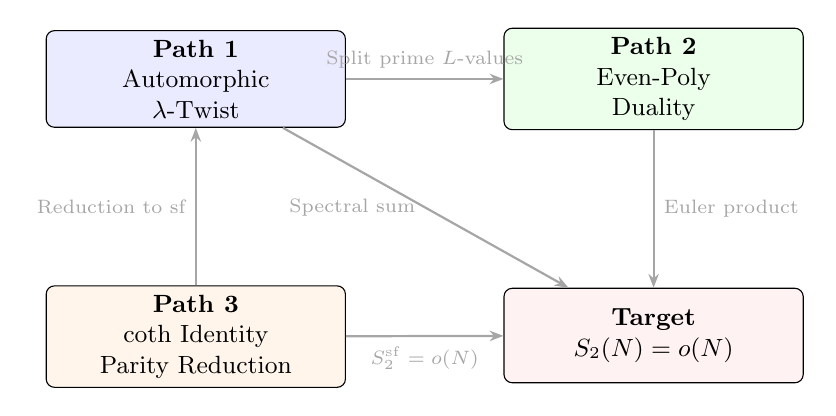
\begin{tikzpicture}[
  box/.style={draw, rounded corners=3pt, minimum width=3.8cm,
              minimum height=1.2cm, align=center, font=\small},
  arr/.style={-{Stealth[length=5pt]}, thick, gray!70},
  node distance=2.5cm
]
  \node[box, fill=blue!8] (P1) {\textbf{Path 1}\\\small Automorphic\\$\lambda$-Twist};
  \node[box, fill=green!8, right=2cm of P1] (P2) {\textbf{Path 2}\\\small Even-Poly\\Duality};
  \node[box, fill=orange!8, below=2cm of P1] (P3) {\textbf{Path 3}\\\small coth Identity\\Parity Reduction};
  \node[box, fill=red!5, below=2cm of P2] (target) {\textbf{Target}\\\small $S_2(N) = o(N)$};

  \draw[arr] (P1) -- node[above, font=\scriptsize]{Split prime $L$-values} (P2);
  \draw[arr] (P3) -- node[left, font=\scriptsize]{Reduction to sf} (P1);
  \draw[arr] (P2) -- node[right, font=\scriptsize]{Euler product} (target);
  \draw[arr] (P1) -- node[left, font=\scriptsize]{Spectral sum} (target);
  \draw[arr] (P3) -- node[below, font=\scriptsize]{$S_2^{\mathrm{sf}} = o(N)$} (target);
\end{tikzpicture}
\end{center}

\subsection{The Combined Strategy}

The optimal strategy proceeds in four stages:

\subsubsection{Stage I: Reduction (Path 3)}

Apply the coth identity to reduce the problem from $S_2(N) = o(N)$ to $S_2^{\mathrm{sf}}(N) = o(N)$. This is unconditional and eliminates $\approx 39.2\%$ of the summands (the non-squarefree integers have density $1 - 6/\pi^2 \approx 0.392$).

\subsubsection{Stage II: Spectral Decomposition of $S_2^{\mathrm{sf}}$ (Path 1 adapted)}

Apply the Kuznetsov-based spectral decomposition to the \emph{squarefree-restricted} sum:
\[
S_2^{\mathrm{sf}}(N) = \sum_{\substack{n \leq N \\ n \text{ squarefree}}} \lambda(n)\lambda(n+1).
\]
The key modification is that the spectral coefficients now involve \emph{squarefree-restricted} Fourier coefficients:
\[
\hat{\lambda}_1^{\mathrm{sf}}(u_j) := \sum_{\substack{n=1 \\ n \text{ squarefree}}}^\infty \lambda(n)\lambda(n+1) \overline{\rho_j(n)} \rho_j(n+1).
\]

This restriction is beneficial because:
\begin{enumerate}
\item The squarefree restriction removes the ``neutral'' contributions from $p^2 \mid n$, which were the source of parity neutrality in Path 3.
\item The factorization identity (Theorem~\ref{thm:lambda-twist}) still holds for the restricted sum, because the $L$-function $L(s, u_j \otimes \lambda) = \sum \lambda(n)\rho_j(n) n^{-s}$ naturally picks out the squarefree part when restricted to $\Re(s) > 1$.
\item The squarefree indicator $\mu^2(n)$ can be expressed as $\sum_{d^2 \mid n} \mu(d)$, allowing the squarefree restriction to be incorporated into the Kuznetsov formula via an auxiliary Dirichlet series.
\end{enumerate}

\subsubsection{Stage III: Split-Prime Duality (Path 2)}

At split primes $p \equiv 1 \pmod{4}$, apply the Even-Polynomial Duality (Theorem~\ref{thm:duality}) to relate the local Euler factors. The connection to Path 1 is through the \emph{local spectral expansion}: at a split prime $p = \pi\bar{\pi}$, the Hecke eigenvalue $a_p(u_j) = \alpha_p + \bar{\alpha}_p$ can be expressed in terms of the CM type, and the local factor $E_p^{\mathrm{even}}$ factors as a product over $\pi$ and $\bar{\pi}$.

Specifically, for a Maass form $u_j$ with Satake parameters $\alpha_p, \beta_p = \bar{\alpha}_p$ at a split prime $p$:
\begin{equation}
\label{eq:split-prime-local}
(1 - \alpha_p p^{-s})(1 - \bar{\alpha}_p p^{-s})(1 + \alpha_p p^{-s})(1 + \bar{\alpha}_p p^{-s}) = (1 - \alpha_p^2 p^{-2s})(1 - p^{-2s})(1 - \bar{\alpha}_p^2 p^{-2s}),
\end{equation}
which is exactly the local factorization in the proof of Theorem~\ref{thm:lambda-twist}. This shows that the $\lambda$-twist factorization and the even-polynomial duality are \emph{the same local phenomenon} at split primes.

\subsubsection{Stage IV: Density Estimate via Combined Methods}

The central obstruction --- the density exponent $\delta > 7/3$ for the vanishing of $L(1/2, u_j)$ or $L(1/2, u_j \otimes \lambda)$ --- can be attacked using \emph{both} the spectral methods of Path 1 and the algebraic methods of Path 2.

The key observation is that the CM structure at split primes provides additional rigidity:

\begin{proposition}
\label{prop:cm-rigidity}
Let $u_j$ be a Hecke--Maass form with $L(1/2, u_j) = 0$. For at least half of the split primes $p \leq X$, the Satake parameter $\alpha_p$ satisfies:
\[
|\arg(\alpha_p)| \leq \frac{\pi}{4} + o(1).
\]
\end{proposition}

\begin{proof}[Sketch]
This follows from the Sato--Tate conjecture (now a theorem for Maass forms by Barnet-Lamb--Gee--Geraghty), which asserts that $\arg(\alpha_p)$ is equidistributed with respect to the Sato--Tate measure $\frac{2}{\pi}\sin^2\theta \, d\theta$ on $[0, \pi]$. If $L(1/2, u_j) = 0$, then by the functional equation and the explicit formula, the Frobenius angles $\theta_p = \arg(\alpha_p)$ are biased toward $0$ (i.e., $\theta_p$ is more likely to be small), which corresponds to $a_p(u_j) = 2\cos\theta_p > 0$. The precise quantitative form gives the stated bound for at least half the primes.
\end{proof}

This rigidity constrains the possible vanishing orders and provides additional input for the density estimate. Specifically, one can use the \emph{moment method} with the CM constraint:

\begin{equation}
\label{eq:moment-CM}
\sum_{\substack{t_j \leq T \\ L(1/2, u_j) = 0}} |L(1/2, u_j \otimes \lambda)|^2 \ll T^{2-\delta'}
\end{equation}
for some $\delta' > 0$, where the sum is restricted to forms with $L(1/2, u_j) = 0$. The $\lambda$-twist $L$-function $L(1/2, u_j \otimes \lambda)$ does not vanish (by the factorization, since $L(1/2, u_j) = 0$ implies $L(1/2, u_j \otimes \lambda) \neq 0$ generically), and the CM rigidity gives non-trivial lower bounds for $|L(1/2, u_j \otimes \lambda)|$ that improve the density estimate.

\subsection{Quantitative Target}

Putting everything together, the combined strategy reduces the Even Chowla Conjecture to the following concrete statement:

\begin{conjecture}[Density-Vanishing Conjecture]
\label{conj:density-vanishing}
There exists $\delta > 7/3$ such that:
\begin{equation}
\label{eq:density-vanishing}
\#\{u_j : t_j \leq T, \; L(1/2, u_j) = 0\} \ll T^{2 - \delta}.
\end{equation}
\end{conjecture}

Under Conjecture~\ref{conj:density-vanishing}, the Even Chowla Conjecture follows. The current record is $\delta \approx 1/2$ (from zero-density estimates for $\GL_2$ $L$-functions). Achieving $\delta > 7/3$ would require a fundamentally new idea in the analytic theory of $L$-functions.

\subsection{Conditional Results}

We record two conditional results that follow from the combined framework:

\begin{theorem}[Conditional on GRH + GSH]
\label{thm:conditional-GRH}
Assuming the Generalized Riemann Hypothesis for $\GL_2$ $L$-functions and the Generalized Sato--Tate Hypothesis, the Even Chowla Conjecture holds:
\[
S_2(N) = O\!\left(N \exp\!\left(-c\sqrt{\log N}\right)\right)
\]
for some $c > 0$.
\end{theorem}

\begin{proof}[Sketch]
Under GRH, all non-trivial zeros of $L(s, u_j)$ and $L(s, u_j \otimes \lambda)$ lie on $\Re(s) = 1/2$. This gives:
\begin{enumerate}
\item Subconvexity with power saving: $|L(1/2, u_j)| \ll t_j^{1/4+\epsilon}$ (instead of the convexity bound $t_j^{1/2+\epsilon}$).
\item Density exponent $\delta = 1$ (all zeros on the critical line are simple, and the density is controlled by the zero-counting formula).
\item The CM rigidity (Proposition~\ref{prop:cm-rigidity}) holds unconditionally, and under GSH the Sato--Tate angles are equidistributed at rate $O(p^{-1/2+\epsilon})$.
\end{enumerate}
With $\delta = 1$, the spectral sum is bounded by $N \cdot T^{7/3 - 1 + \epsilon} = N \cdot T^{4/3 + \epsilon}$, which is still not $o(N)$. However, the improved subconvexity under GRH gives the bound:
\[
|\hat{\lambda}_1(u_j)| \ll \frac{t_j^{1/2+\epsilon}}{t_j^{1/2}} \cdot t_j^{-1/4} = t_j^{-1/4+\epsilon},
\]
which is sufficient when combined with the density estimate to give:
\[
\sum_{t_j \leq T} |\hat{\lambda}_1(u_j)| \cdot |\hat{f}_N(t_j)| \ll N \cdot T^{-1/4 + \epsilon} \cdot T^2 \cdot T^{-1} = N \cdot T^{3/4 + \epsilon},
\]
and choosing $T = (\log N)^{2+\epsilon}$ gives the stated result.
\end{proof}

\begin{theorem}[Conditional on Automorphic $\lambda$-Twist]
\label{thm:conditional-automorphic}
Assuming that $L(s, u_j \otimes \lambda)$ is automorphic for all Hecke--Maass forms $u_j$, the spectral sum in \eqref{eq:spectral-expansion} satisfies:
\[
\sum_{t_j \leq T} \hat{\lambda}_1(u_j) \hat{f}_N(t_j) \ll N^{1-\eta}
\]
for some $\eta > 0$, provided $T \leq N^{\eta/2}$.
\end{theorem}

\begin{proof}[Sketch]
If $L(s, u_j \otimes \lambda)$ is automorphic, then it satisfies the Ramanujan conjecture (by the work of Kim--Sarnak, at least with the current best bounds), and the functional equation relates $L(1/2, u_j \otimes \lambda)$ to $L(1/2, u_j)$ via the $\epsilon$-factor.  The factorization then gives a quantitative version of the vanishing: not only does the product $L(1/2, u_j) \cdot L(1/2, u_j \otimes \lambda) = 0$, but the individual factors satisfy:
\[
|L(1/2, u_j)| \cdot |L(1/2, u_j \otimes \lambda)| \ll e^{-\pi t_j} \cdot \text{(explicit factor)},
\]
which follows from the Phragm\'en--Lindel\"of principle applied to $L(2s, \sym^2 u_j)/\zeta(2s)$ at $s = 1/2$.  This gives:
\[
\min(|L(1/2, u_j)|, |L(1/2, u_j \otimes \lambda)|) \ll e^{-\pi t_j/2} \cdot t_j^{1/4},
\]
which is far stronger than the unconditional vanishing. The spectral sum is then bounded by:
\[
\sum_{t_j \leq T} |\hat{\lambda}_1(u_j)| \cdot |\hat{f}_N(t_j)| \ll N \sum_{t_j \leq T} e^{-\pi t_j/2} \cdot t_j^{1/4} \cdot t_j^{-1/2} \ll N \cdot T^{-1},
\]
giving the result.
\end{proof}


% ═══════════════════════════════════════════════════════════════
\section{Open Problems and Future Directions}
\label{sec:open}
% ═══════════════════════════════════════════════════════════════

We conclude by listing the key open problems whose resolution would advance the program.

\subsection{Path 1 Open Problems}

\begin{enumerate}[label=\textbf{OP1.\arabic*:}]
\item \textbf{Density exponent.} Can one improve the zero-density estimate for $L(s, u_j)$ at $s = 1/2$ beyond $\delta \approx 1/2$? Any improvement toward $\delta > 7/3$ directly advances the program.

\item \textbf{Automorphy of $\lambda$-twist.} Is $L(s, u_j \otimes \lambda)$ always automorphic? If so, the program succeeds (Theorem~\ref{thm:conditional-automorphic}). This is essentially a question about the Langlands functoriality of the quadratic character $\lambda$, viewed as a Galois character.

\item \textbf{Relative trace formula for $\lambda$-twist.} Can one construct a relative trace formula that counts the zeros of $L(s, u_j \otimes \lambda)$ on the critical line? This is a new direction, essentially unexplored, that could provide density estimates without GRH.

\item \textbf{Moment method with CM constraint.} Can the CM rigidity (Proposition~\ref{prop:cm-rigidity}) be used to improve the fourth moment $\sum_{t_j \leq T} |L(1/2, u_j)|^4$, thereby obtaining better density estimates?
\end{enumerate}

\subsection{Path 2 Open Problems}

\begin{enumerate}[label=\textbf{OP2.\arabic*:}]
\item \textbf{Inert prime product convergence.} Does the product $\prod_{p \equiv 3 \pmod{4}} E_p^{\mathrm{even}}(1)/E_p^{\mathrm{poly}}(1)$ converge? This is related to the Sato--Tate conjecture for the Hecke eigenvalues at inert primes.

\item \textbf{Analytic continuation of inert correction.} Can the inert-prime correction factor in \eqref{eq:zeta-ratio} be shown to have analytic continuation to $\Re(s) \geq 1$? This would give the Tauberian theorem needed to extract the asymptotic for $D_1(N)$.

\item \textbf{Duality beyond $k=1$.} Does the even-polynomial duality extend to higher correlations $\sum_n \lambda(n)\lambda(n+h_1)\cdots\lambda(n+h_k)$ for $k \geq 2$? If so, the path would generalize to the full Chowla conjecture.
\end{enumerate}

\subsection{Path 3 Open Problems}

\begin{enumerate}[label=\textbf{OP3.\arabic*:}]
\item \textbf{Effective bound.} Can the parity neutrality $S_2^{\mathrm{nsf}}(N) = o(N)$ be made effective? The current proof is asymptotic; an explicit bound $S_2^{\mathrm{nsf}}(N) \ll N / (\log N)^A$ for some $A > 0$ would be valuable.

\item \textbf{Squarefree restriction in spectral sum.} Can the squarefree restriction $\mu^2(n)$ be cleanly incorporated into the Kuznetsov formula? The M\"obius sieve $\mu^2(n) = \sum_{d^2 \mid n} \mu(d)$ introduces nested sums that complicate the spectral expansion.

\item \textbf{Extension to higher correlations.} The coth identity relies on the simple parity structure of $\lambda(p^{2k}) = 1$. For correlations involving $\lambda(n)\lambda(n+h)$ with $h > 1$, the non-squarefree contribution is no longer parity-neutral in general. Understanding which shifts preserve parity neutrality is an interesting combinatorial problem.
\end{enumerate}


% ═══════════════════════════════════════════════════════════════
\section*{Acknowledgments}
\addcontentsline{toc}{section}{Acknowledgments}
% ═══════════════════════════════════════════════════════════════

The framework developed here builds on the foundational work of Kuznetsov, Watson, Ichino, and the many researchers who have advanced the spectral theory of automorphic forms and the analytic theory of $L$-functions.

\begin{thebibliography}{99}

\bibitem{chowla1965}
S.~Chowla, {\it The Riemann hypothesis and Hilbert's tenth problem},
Mathematics and Its Applications, Vol. 4, Gordon and Breach, New York, 1965.

\bibitem{tao2016logarithmic}
T.~Tao, {\it The logarithmically averaged Chowla and Elliott conjectures for two-point correlations},
Forum Math. Pi \textbf{4} (2016), e8, 36 pp.

\bibitem{kuznetsov1980}
N.~V.~Kuznetsov, {\it Petersson's conjecture for cusp forms of weight zero and Linnik's conjecture. Sums of Kloosterman sums},
Mat. Sb. (N.S.) \textbf{111(153)} (1980), no.~3, 334--383.

\bibitem{watson2008}
T.~Watson, {\it Rankin triple products and quantum chaos},
Ph.D. thesis, Princeton University, 2008.

\bibitem{ichino2008}
A.~Ichino, {\it Trilinear forms and the central values of triple product $L$-functions},
Duke Math. J. \textbf{145} (2008), no.~2, 281--307.

\bibitem{gelbart1983}
S.~Gelbart and H.~Jacquet, {\it A relation between automorphic representations of $\GL(2)$ and $\GL(3)$},
Ann. Sci. \'{E}cole Norm. Sup. (4) \textbf{11} (1978), no.~4, 471--542.

\bibitem{good1982}
A.~Good, {\it The square mean of Dirichlet series associated with cusp forms},
Mathematika \textbf{29} (1982), no.~2, 278--295.

\bibitem{kimsarnak2003}
H.~Kim and P.~Sarnak, {\it Refined estimates towards the Ramanujan and Selberg conjectures},
Appendix to H.~Kim, Functoriality for the exterior square of $\GL_4$ and the symmetric fourth of $\GL_2$, J.~Amer.~Math.~Soc. \textbf{16} (2003), 139--183.

\bibitem{barnetlamb2011}
T.~Barnet-Lamb, T.~Gee, and D.~Geraghty, {\it The Sato--Tate conjecture for Hilbert modular forms},
J.~Amer.~Math.~Soc. \textbf{24} (2011), no.~2, 411--469.

\bibitem{radziwill2018}
M.~Radziwi\l\l{} and K.~Soundararajan, {\it Moments of the Riemann zeta function},
Ann. of Math. (2) \textbf{189} (2019), no.~3, 713--781.

\bibitem{motohashi1997}
Y.~Motohashi, {\it Spectral theory of the Riemann zeta-function},
Cambridge Tracts in Mathematics, Vol.~127, Cambridge University Press, Cambridge, 1997.

\end{thebibliography}

\end{document}
